\documentclass{beamer}
\usetheme{Warsaw}
\useinnertheme{circles}
\useoutertheme[subsection=false]{smoothbars}
\usepackage[utf8x]{inputenc}
\usepackage[czech]{babel}
\usepackage[T1]{fontenc}
\usepackage{listings}
\usepackage{tikz}
\lstset{basicstyle=\tiny\ttfamily}
\logo{
\includegraphics[height=0.5cm]{brmlab.pdf}}

\begin{document}

\AtBeginSection[]
{
  \begin{frame}
    \frametitle{Outline}
    \tableofcontents[currentsection]
  \end{frame}
}

\title{brmiversity: Umělá inteligence \\ a teoretická informatika}
\subtitle{Přednáška č. 9}
\author{Petr Baudiš $\langle${\tt pasky@ucw.cz}$\rangle$}
\institute{
	brmlab 2011\\
	\vskip 1ex
	\pgfdeclareimage[height=4ex]{ccbysa}{by-sa.pdf}
	\pgfuseimage{ccbysa}
}
\date{}
\frame{\titlepage}

\section{Umělá inteligence}

\subsection{}
\begin{frame}{Strojové učení}
\begin{center}
Učící se agent: Datový vstup a výstup, rozhodovací problém, užitková funkce
\vskip 3ex
\begin{block}{Máme trénovací množinu}
\begin{itemize}
\item Učení s učitelem vs. bez učitele
\item Rozpoznávání vs. samoorganizace
\end{itemize}
\end{block}
\begin{block}{Nemáme trénovací množinu}
\begin{itemize}
\item Exploration---exploitation dilemma
\item Zpětnovazebné učení
\end{itemize}
\end{block}
\end{center}
\end{frame}

\subsection{}
\begin{frame}{Strojové učení nad daty}
\begin{center}
Dnes: Máme trénovací a testovací data, hledáme {\em hypotézu}. \\
Chceme řešit buď {\em klasifikační} nebo {\em regresní} úlohy. \\
Parametrické vs. samplovací metody.
\vskip 3ex
\begin{block}{Učení s učitelem}
\begin{itemize}
\item Prohledávání prostoru verzí
\vskip 2ex
\item {\bf Rozhodovací stromy}
\item {\bf Bayesovské učení}
\item Částicové filtry
\vskip 2ex
\item Neuronové sítě
\item {\bf Support Vector Machines}
\end{itemize}
\end{block}
\begin{block}{Učení bez učitele}
\begin{itemize}
\item Karuhnenova-Loèveho transformace (PCA)
\item {\bf Clusterování}
\item Kohonenovy mapy
\item Lineární regrese
\end{itemize}
\end{block}
\end{center}
\end{frame}

\subsection{}
\begin{frame}{Rozhodovací stromy}
\begin{itemize}
\item Struktura
\item Informační entropie
\item ID3
\end{itemize}
\end{frame}

\subsection{}
\begin{frame}{Bayesovské učení}
\begin{itemize}
\item Nasbírané pravděpodobnosti, věrohodnost
\item Bayesovo pravidlo
\item Predikce
\item Preference jednoduchých hypotéz
\item MAP, MDL, ML (maximální věrohodnost)
\end{itemize}
\end{frame}

\subsection{}
\begin{frame}{Naivní Bayesovský klasifikátor}
\begin{itemize}
\item Předpoklad --- podmíněná nezávislost
\item Predikční pravidlo
\item Spamfilter
\end{itemize}
\begin{block}{EM algoritmus}
\begin{itemize}
\item Estimation-maximization, střídáme kroky
\end{itemize}
\end{block}
\end{frame}

\subsection{}
\begin{frame}{Support Vector Machines}
\begin{itemize}
\item Kernelová metoda používající reprezentanty
\item Lineární separace nejširším okrajem
\item Remapování neseparabilních množin kernelem
\end{itemize}
\end{frame}

\subsection{}
\begin{frame}{Clusterování}
\begin{itemize}
\item $k$-means
\item Hierarchické shlukování
\item Evoluční stromy
\end{itemize}
\end{frame}

\subsection{}
\begin{frame}{Otázky?}
\begin{center}
Příště: Strojové učení zkušeností.
\end{center}
\end{frame}

\section{Neuronové sítě}

\subsection{}
\begin{frame}{Asociativní paměti}
\begin{itemize}
\item Umělé neurony (``výpočetní krabičky'') \\ dostávají vstupy (čísla) a na jejich \\ základě generují výstup (číslo)
\item Dříve: Vrstvy striktně oddělené, \\ vstupní vrstva se vstupy zvnějšku, \\ výstupní vrstva s výstupem pro uživatele, \\ skryté vrstvy vyhodnocují různé charakteristiky vstupů
\item Dnes: Jinak! 2D síť neuronů se zpětnými spoji.
	TODO
\end{itemize}
\begin{tikzpicture}[remember picture,overlay]
  \node [xshift=-4.5cm,yshift=-6cm,above right] at (current page.north east)
    {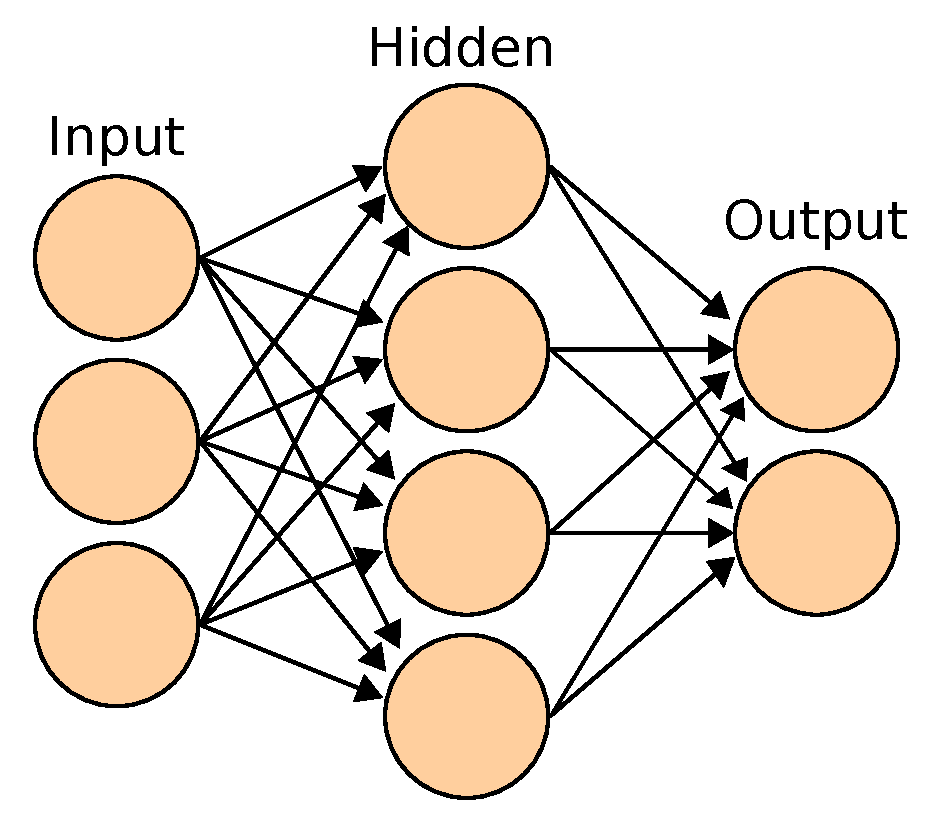
\includegraphics[width=4cm]{ANN.pdf}};
\end{tikzpicture}
\end{frame}

\subsection{}
\begin{frame}{Model asociativní paměti}
\begin{itemize}
\item BAM
\item Hebbovské učení
\item Energetická funkce
\end{itemize}
\end{frame}

\subsection{}
\begin{frame}{Hopfieldova síť}
\begin{itemize}
\item Reprezentace, vyhodocování, učení
\end{itemize}
\end{frame}

\subsection{}
\begin{frame}{Reprezentace úloh}
\begin{itemize}
\item TSP jako energetická funkce
\end{itemize}
\end{frame}

\subsection{}
\begin{frame}{Stochastické učení}
\begin{itemize}
\item Simulated annealing
\end{itemize}
\end{frame}

\subsection{}
\begin{frame}{Otázky?}
\begin{center}
Příště: Samoorganizace v rámci ANN.
\end{center}
\end{frame}

\section{Evoluční algoritmy}

\subsection{}
\begin{frame}{Rekapitulace --- genetický algoritmus}
\begin{itemize}
\item Populace řešení (s určitou strukturou), ohodnocovací funkce
\item Máme populaci předchozí generace, vyrábíme novou generaci (dokud nenajdeme optimum).
\item Nová generace (dokud není plná) --- aplikuj genetické operátory:
\begin{itemize}
\item Vyber dva jedince z minulé populace (selekce)
\item Vyrob dva nové jedince (křížení)
\item Mírně jedince uprav (mutace)
\item Dvojici vlož do nové generace
\end{itemize}
\end{itemize}
\end{frame}

\subsection{}
\begin{frame}{Reprezentační schémata}
\begin{itemize}
\item Definice schémat
\item Věta o schématech
\end{itemize}
\end{frame}

\subsection{}
\begin{frame}{Evoluční programování}
\begin{itemize}
\item Programování evoluce
\item Dynamická změna parametrů GA
\end{itemize}
\end{frame}

\subsection{}
\begin{frame}{Genetické programování}
\begin{itemize}
\item Rosteme LISP
\end{itemize}
\end{frame}

\subsection{}
\begin{frame}{Otázky?}
\begin{center}
Příště: Koevoluce a otevřená evoluce (brmlife). \\ Pravděpodobnostní model GA.
\end{center}
\end{frame}

\section{Datové struktury}

\subsection{}
\begin{frame}{Haldy}
\begin{itemize}
\item Rekapitulace
\item Levicové haldy
\item Binomiální haldy
\item Fibonacciho haldy
\end{itemize}
\end{frame}

\subsection{}
\begin{frame}{Binární vyhledávací strom}
\begin{itemize}
\item TODO: obrazek
\item Binární strom --- hrany pouze ``směrem dolů'', jeden kořen, každý uzel má nula (list) až dva syny
\item Vyhledávací strom --- vše v levém podstromu $\le n \le $ vše v pravém podstromu
\item Vyhledávání --- cesta z kořenu k uzlu
\item Vnitřní uzly --- data nebo navigace?
\item Jak vyrobit strom nad datasetem?
\vskip 3ex
\pause
\item Vyvážený strom --- hloubky podstromů se liší jenom málo
\item Ve vyváženém stromě trvá hledání $O(\log n)$
\item Jak vyrobit vyvážený strom nad datasetem?
\pause
\item Jak ho udržovat vyvážený?
\pause
\item Chceme operace INSERT, DELETE
\item Naivně: INSERT do listu, rotace u DELETE
\end{itemize}
\end{frame}

\subsection{}
\begin{frame}{Stromy rovnoměrně rozložených hodnot}
\begin{itemize}
\item Hodnoty jsou rovnoměrně rozložené (třeba hashe)
\item Je potřeba vůbec vyvažovat?
\end{itemize}
\end{frame}

\subsection{}
\begin{frame}{Splay stromy}
\begin{itemize}
\item Zavedeme operaci {\em splay} --- rotaci uzlu zevnitř stromu do kořene
\item INSERT --- do listu a splay
\item DELETE --- splay rodiče a utrhnout
\item FIND --- splay do kořene
\item Asymptoticky vyvážený strom!
\end{itemize}
\end{frame}

\subsection{}
\begin{frame}{Červeno-černé stromy}
\begin{itemize}
\item Některé vnitřní uzly červeně {\em obarvíme}; barvy opatrně střídáme
\item Přesná konstrukce
\end{itemize}
\end{frame}

\subsection{}
\begin{frame}{AVL stromy}
\begin{itemize}
\item Konstrukce, vlastnosti
\end{itemize}
\end{frame}

\subsection{}
\begin{frame}{Otázky?}
\begin{center}
Příště: B-stromy.
\end{center}
\end{frame}

\subsection{}
\begin{frame}{Děkuji vám}
\begin{center}
{\bf pasky@ucw.cz}

\vskip 6ex

Příště: Strojové učení podle zkušeností --- v umělé inteligenci obecně a~v~rámci adaptivních agentů. \\
	Neuronové sítě.
	Datové struktury.
\end{center}
\end{frame}

\end{document}
